\documentclass{report}
\usepackage[margin=1in, paperwidth=8.5in, paperheight=11in]{geometry}
%Math packages%
\usepackage{amsmath}
\usepackage{amsthm}
%Spacing%
\usepackage{setspace}
\onehalfspacing
%Lecture number%
\newcommand{\lectureNum}{10}
%Variables - Date and Course%
\newcommand{\curDate}{February 2, 2017}
\newcommand{\course}{CS 241}
\newcommand{\instructor}{Kevin Lanctot}
%Defining the example tag%
%\theoremstyle{definition}%
\newtheorem{ex}{Example}[section]
%Setting counter given the lecture number%
\setcounter{chapter}{\lectureNum{}}
%Package to insert code%
\usepackage{listings}
\usepackage{courier}
\usepackage{xcolor}
\lstset { %
    tabsize=2,
    breaklines=true,
    language=C++,
    backgroundcolor=\color{blue!8}, % set backgroundcolor
    basicstyle=\footnotesize\ttfamily,% basic font setting
}
%Package for images%
\usepackage{graphicx}

\begin{document}
%Note title%
\begin{center}
\begin{Large}
\textsc{\course{} | Lecture \lectureNum{}}
\end{Large}
\end{center} 
\noindent \textit{Bartosz Antczak} \hfill
\textit{Instructor: \instructor{}} \hfill
\textit{\curDate{}}
\rule{\textwidth}{0.4pt}
% Actual Notes%
\section{Finite Automata}
This is also known as a deterministic \textit{finite state machine} (FSM). It's comprised of:
\begin{itemize}
\item A finite set of states which includes a start state and at least one \textit{accepting states}
\item A finite set of input symbols
\item A finite set of transitions
\end{itemize}
The \textit{deterministic finite automata} (DFA) determines if input is accepted (e.g., is a word in a language) or rejected (e.g., the word is not in the language).
\begin{ex}
A deterministic finite automata of a sample person's daily routine
\end{ex}
\begin{figure}[ht]
\begin{center}
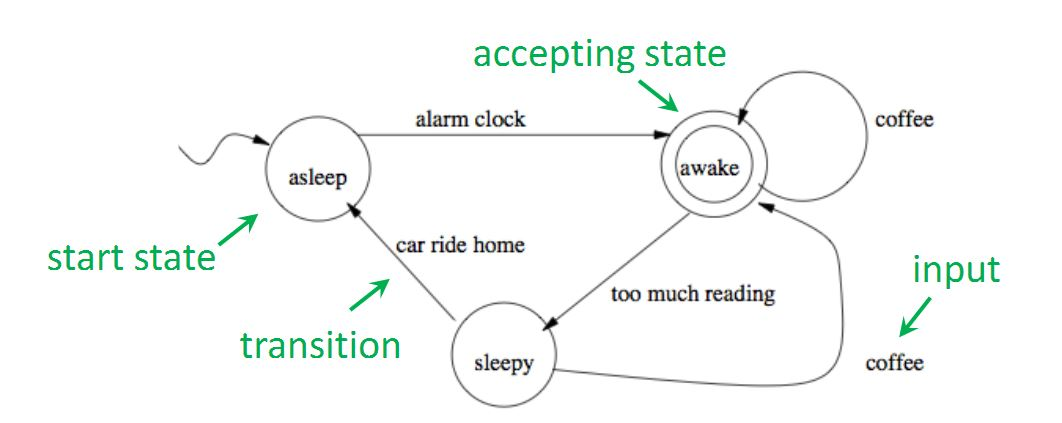
\includegraphics[scale=0.5]{fsm1.jpg}
\end{center}
\caption{Courtesy from Prof. Lanctot's slides}
\end{figure}
A DFA contains:
\begin{itemize}
\item \textbf{States} (drawn as circles): there are two types
\begin{itemize}
\item \textit{start state:} denoted with a curved line
\item \textit{accepting state(s):} denoted as two concentric circles
\end{itemize}
We can label these states, but that's optional\newpage
\item \textbf{Transitions:} an edge that moves from one state to another
\begin{figure}[ht]
\begin{center}
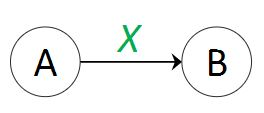
\includegraphics[scale=0.5]{input1.jpg}
\end{center}
\caption{This means: \textit{on input X, move from state A to state B}. If the input does not match any of the possible transitions, an error is thrown. Courtesy from Prof. Lanctot's slides}
\end{figure}
\end{itemize}
\subsubsection{Comparison to Programming Languages}
The components of finite automata can be linked to what you would see in a program:
\begin{figure}[ht]
\begin{center}
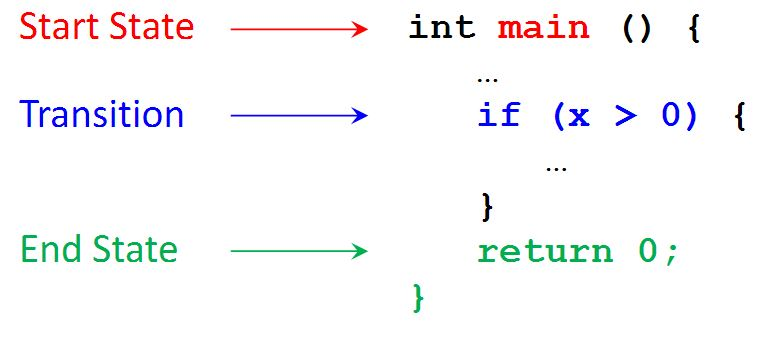
\includegraphics[scale=0.3]{code.jpg}
\end{center}
\caption{Courtesy from Prof. Lanctot's slides}
\end{figure}
\subsection{Examples of DFAs}
Let $\Sigma = \{a, b, c\}$
\subsubsection{Exercise 1}
Create a regular expression and a DFA that accepts the language of strings that contain exactly one $a$, one $b$, and no $c$'s.\\
The language is \{$ab, ba$\}. The DFA is:
\begin{figure}[ht]
\begin{center}
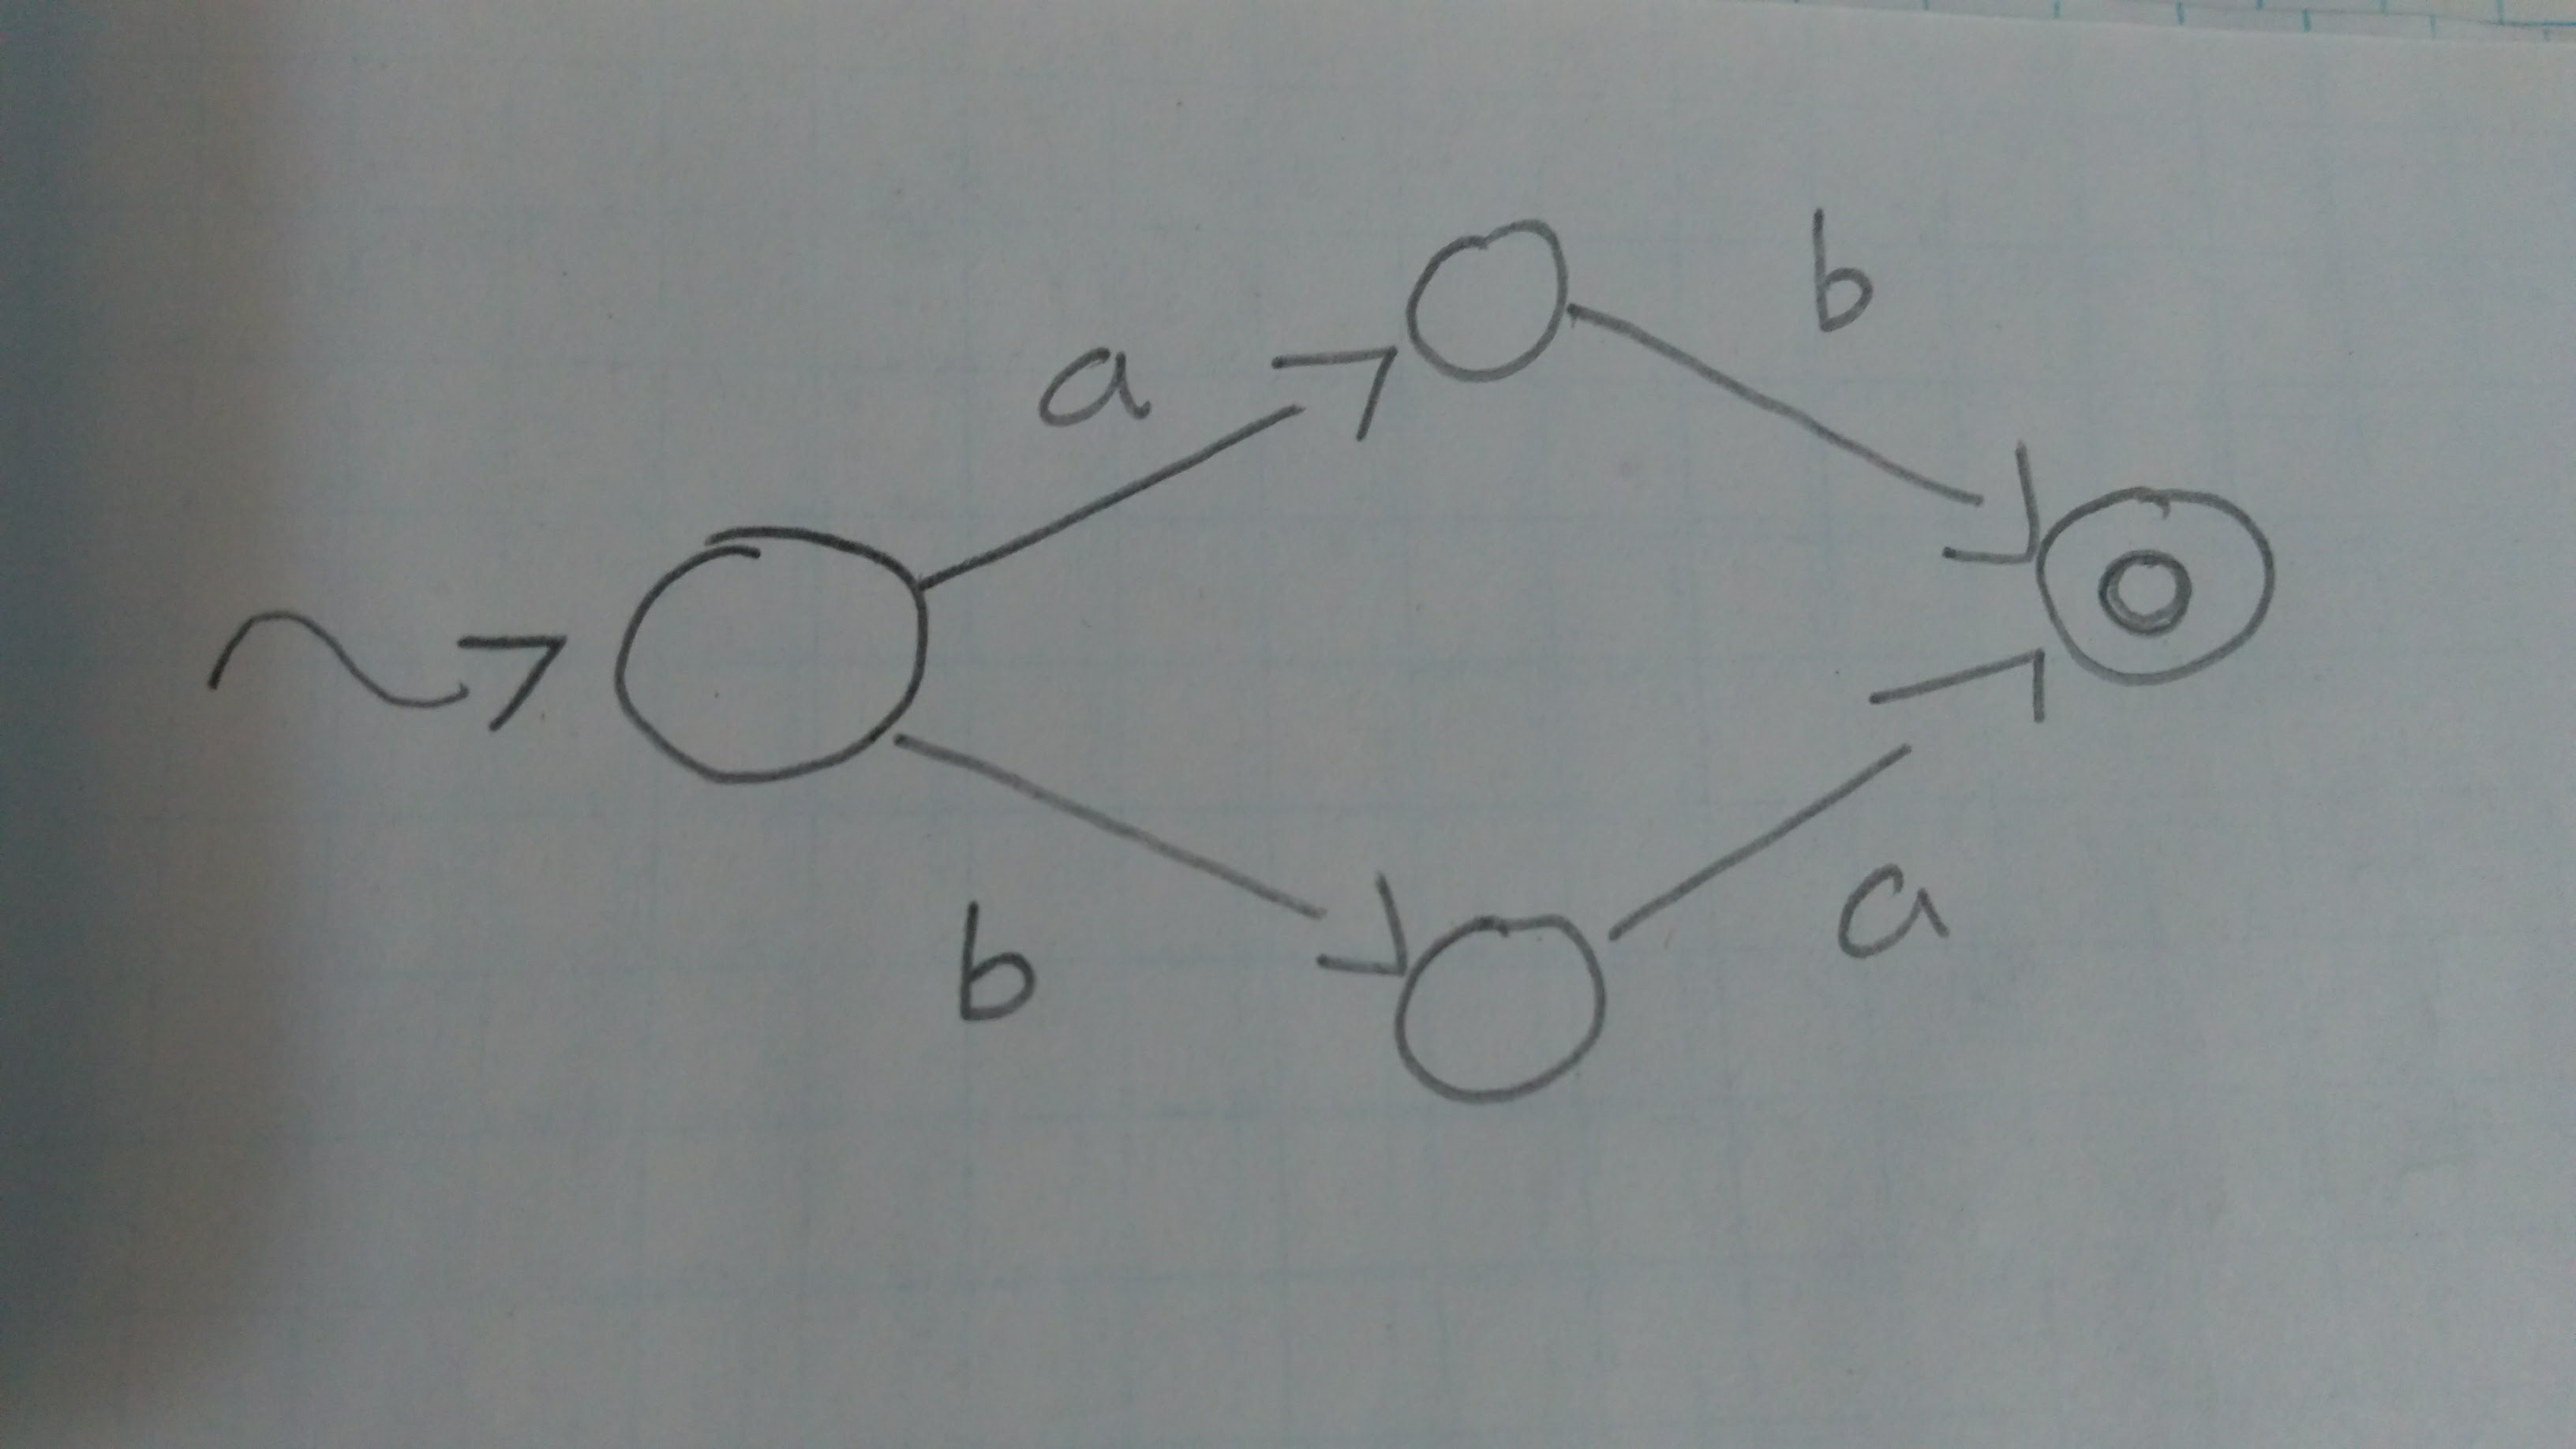
\includegraphics[scale=0.08]{dfa1.jpg}
\end{center}
\end{figure}
\subsubsection{Exercise 2}
Create a regular expression and a DFA that accepts the language of strings that contain at least one $a$.\\
The regular expression is $(b\vert c)^*a(a|b|c)^*$ (the string starts with $b$ or $c$, then contains one $a$, then is followed by any letter in the language). The DFA is:
\begin{figure}[ht]
\begin{center}
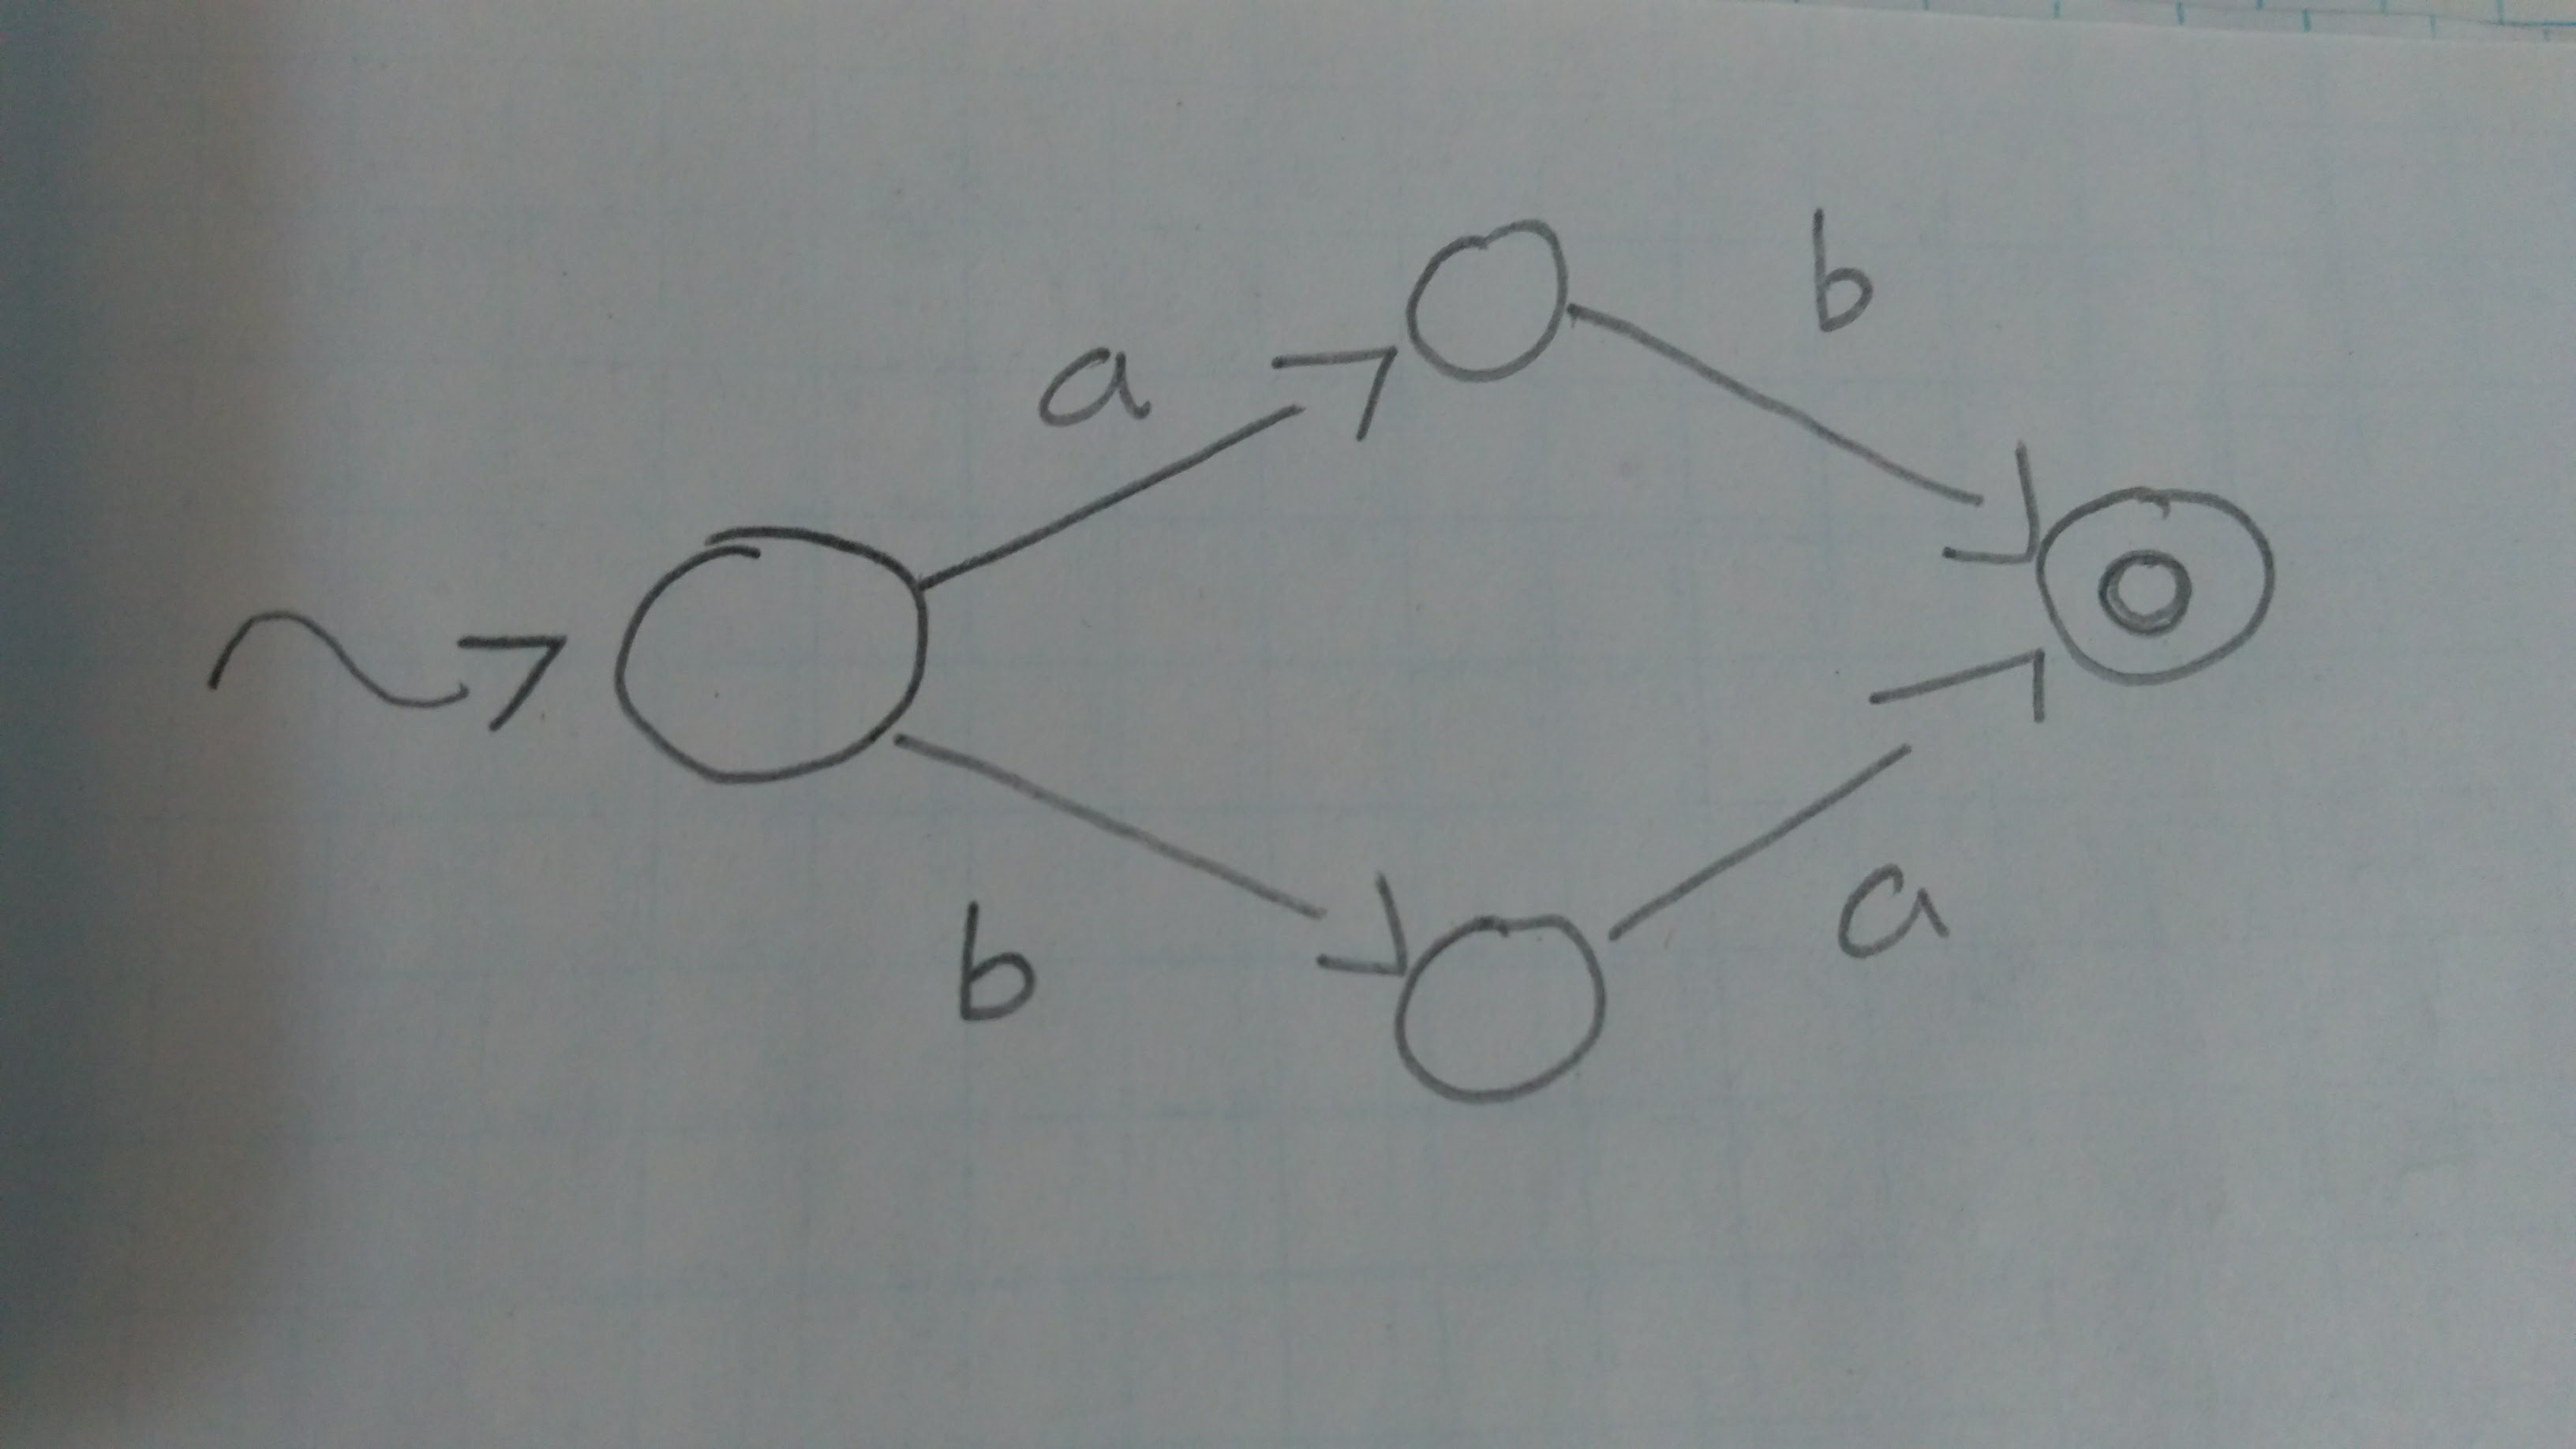
\includegraphics[scale=0.08]{dfa1.jpg}
\end{center}
\end{figure}
\subsubsection{Exercise 3}
Create a DFA that accepts the language of strings that contain an even number of $a$'s (including 0 $a$'s). The DFA is:
\begin{figure}[ht]
\begin{center}
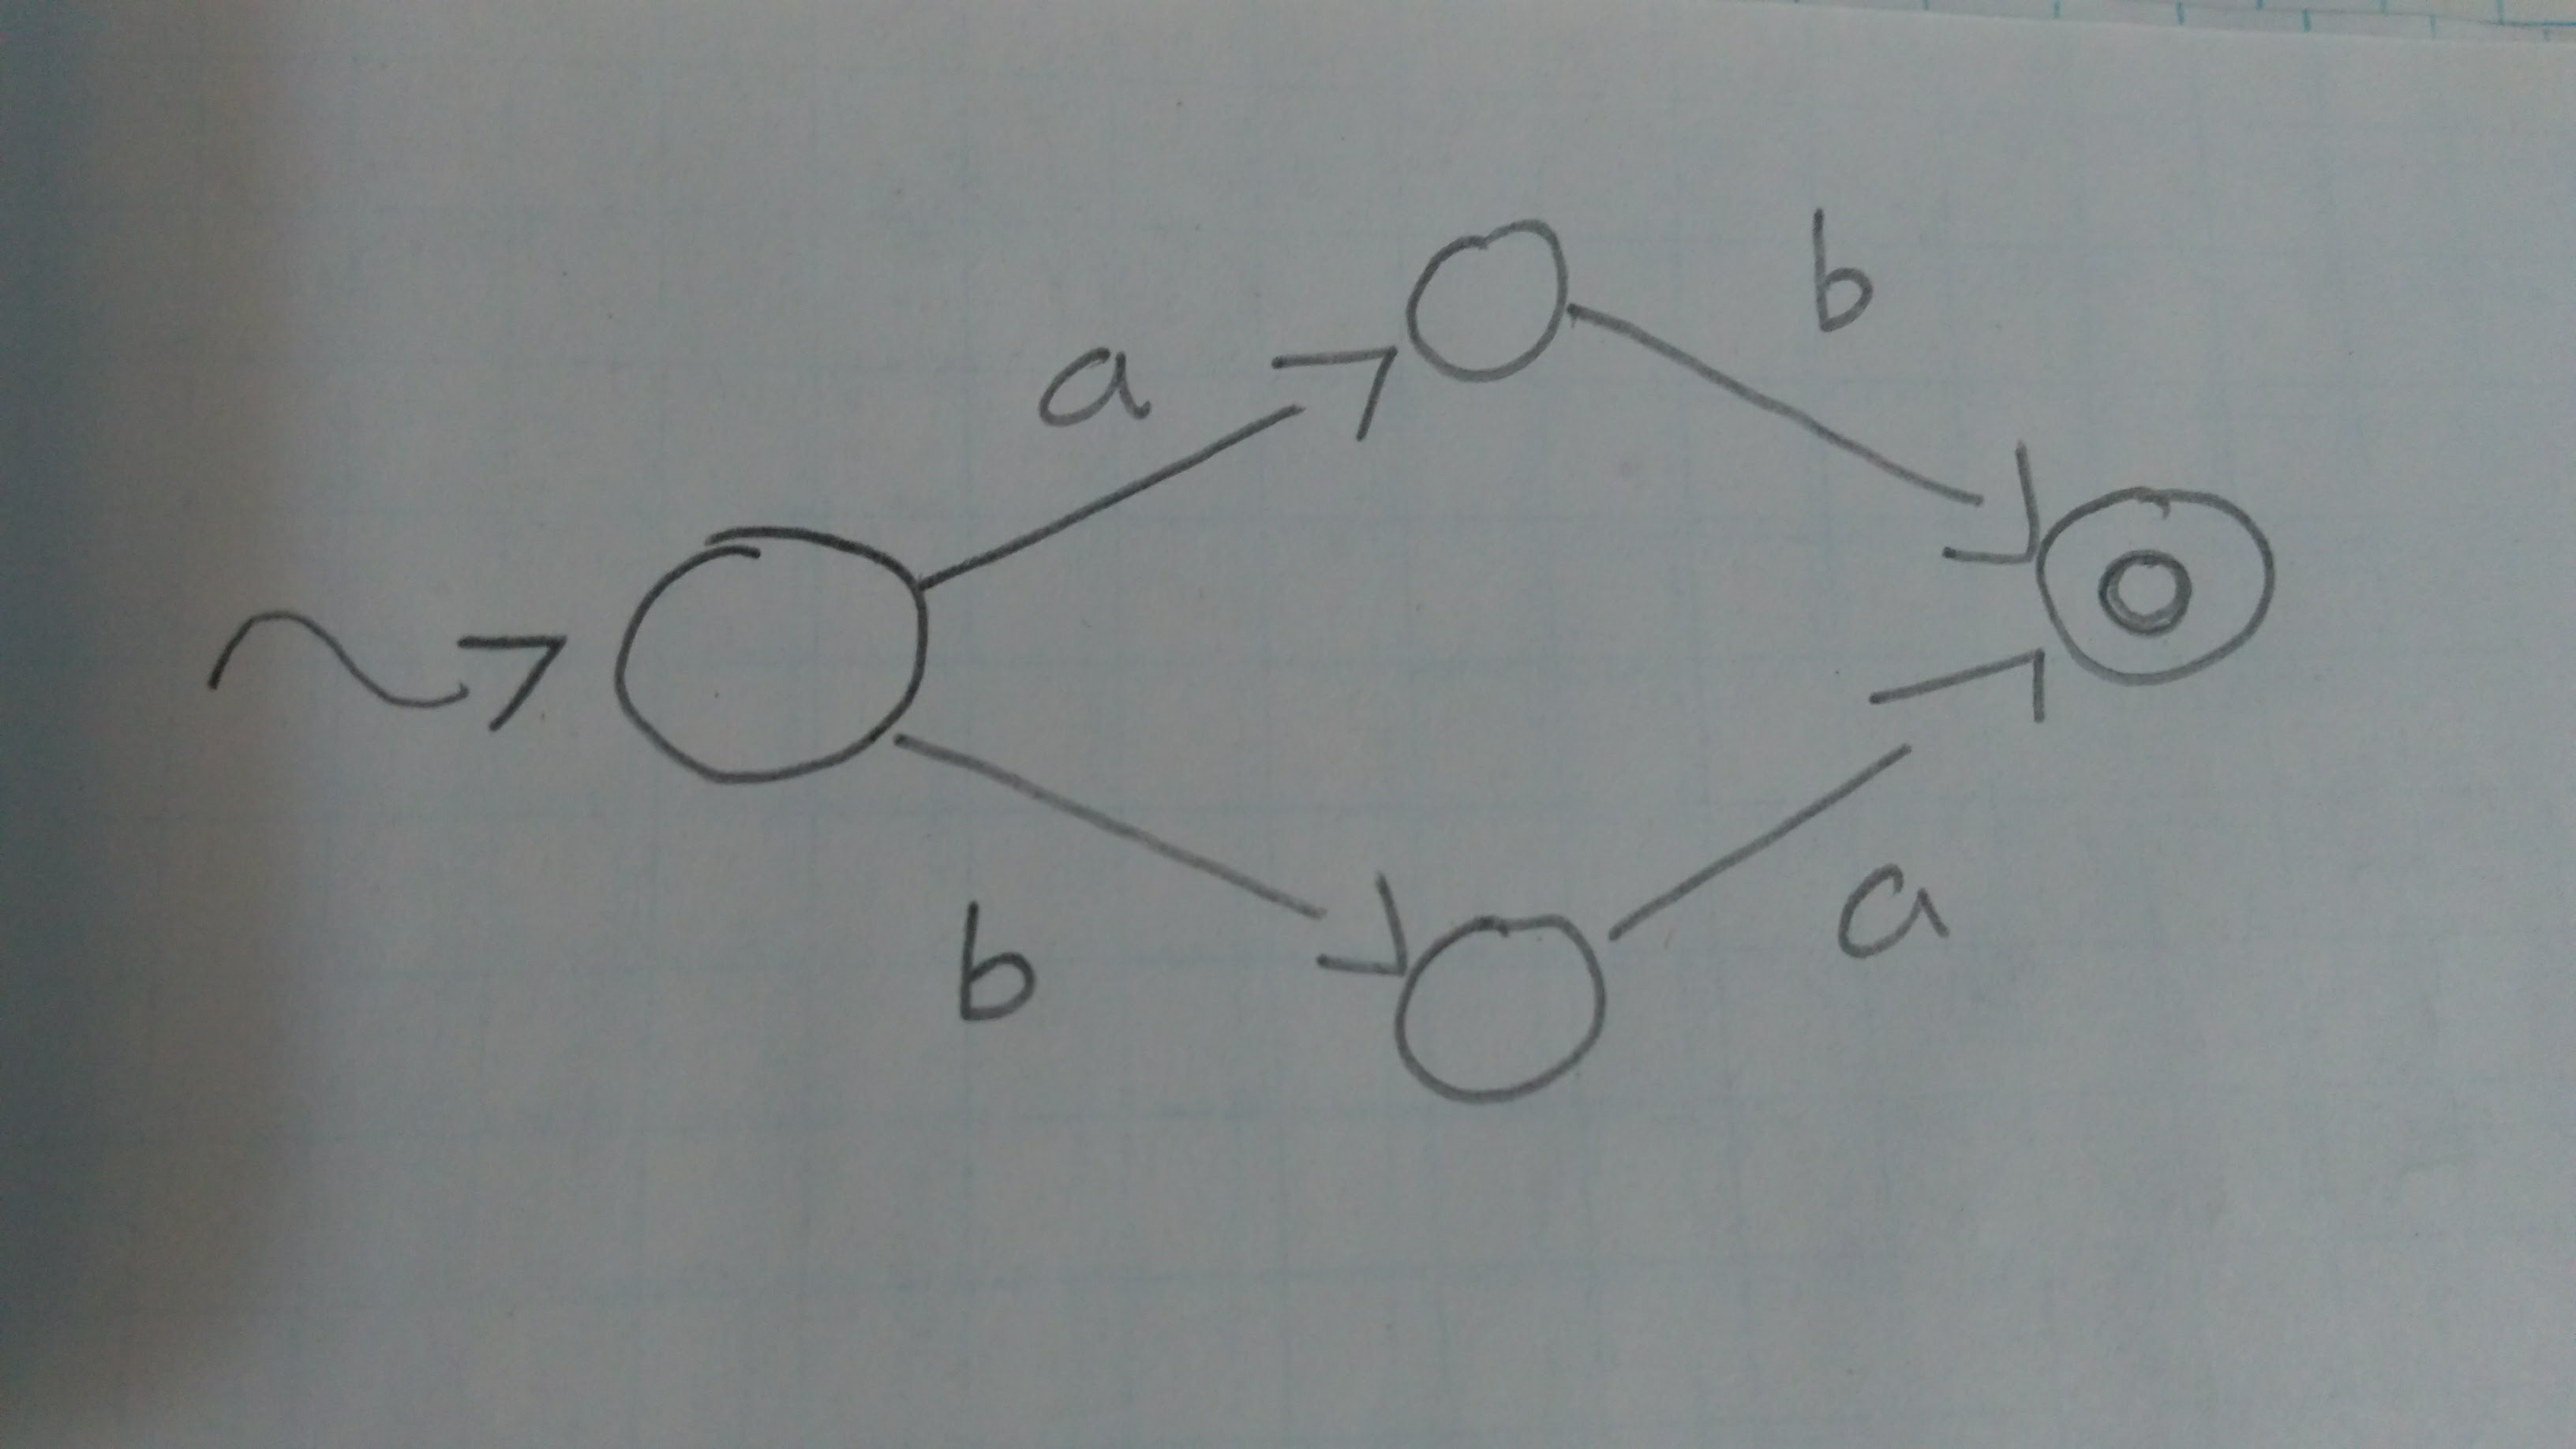
\includegraphics[scale=0.08]{dfa1.jpg}
\end{center}
\end{figure}.
\subsection{Formal Definition of a DFA}
A DFA is a 5-tuple $(\Sigma, Q, q_0, A, \delta)$, where
\begin{itemize}
\item $\Sigma$ is a finite alphabet, e.g., $\Sigma = \{b, e, n, q\}$
\item $Q$ is a finite set of states, e.g., $Q = \{S, b, be, bn, beq, bne\}$
\item $q_0$ is the start state, e.g., $q_0 = \{S\}$
\item $A$ is the set of accepting states, e.g., $A = \{beq, bne\}$
\item $\delta$ is the transition function that maps the pair of state and symbol to state. Denoted as $\delta(Q, \Sigma) = \Sigma^\prime$.
\end{itemize}
%END%
\end{document}